\documentclass[]{article}
\usepackage{lmodern}
\usepackage{amssymb,amsmath}
\usepackage{ifxetex,ifluatex}
\usepackage{fixltx2e} % provides \textsubscript
\ifnum 0\ifxetex 1\fi\ifluatex 1\fi=0 % if pdftex
  \usepackage[T1]{fontenc}
  \usepackage[utf8]{inputenc}
\else % if luatex or xelatex
  \ifxetex
    \usepackage{mathspec}
  \else
    \usepackage{fontspec}
  \fi
  \defaultfontfeatures{Ligatures=TeX,Scale=MatchLowercase}
  \newcommand{\euro}{€}
\fi
% use upquote if available, for straight quotes in verbatim environments
\IfFileExists{upquote.sty}{\usepackage{upquote}}{}
% use microtype if available
\IfFileExists{microtype.sty}{%
\usepackage{microtype}
\UseMicrotypeSet[protrusion]{basicmath} % disable protrusion for tt fonts
}{}
\usepackage[margin=1in]{geometry}
\usepackage{hyperref}
\PassOptionsToPackage{usenames,dvipsnames}{color} % color is loaded by hyperref
\hypersetup{unicode=true,
            pdftitle={Math 141 KEY},
            pdfborder={0 0 0},
            breaklinks=true}
\urlstyle{same}  % don't use monospace font for urls
\usepackage{graphicx,grffile}
\makeatletter
\def\maxwidth{\ifdim\Gin@nat@width>\linewidth\linewidth\else\Gin@nat@width\fi}
\def\maxheight{\ifdim\Gin@nat@height>\textheight\textheight\else\Gin@nat@height\fi}
\makeatother
% Scale images if necessary, so that they will not overflow the page
% margins by default, and it is still possible to overwrite the defaults
% using explicit options in \includegraphics[width, height, ...]{}
\setkeys{Gin}{width=\maxwidth,height=\maxheight,keepaspectratio}
\setlength{\parindent}{0pt}
\setlength{\parskip}{6pt plus 2pt minus 1pt}
\setlength{\emergencystretch}{3em}  % prevent overfull lines
\providecommand{\tightlist}{%
  \setlength{\itemsep}{0pt}\setlength{\parskip}{0pt}}
\setcounter{secnumdepth}{0}

%%% Use protect on footnotes to avoid problems with footnotes in titles
\let\rmarkdownfootnote\footnote%
\def\footnote{\protect\rmarkdownfootnote}

%%% Change title format to be more compact
\usepackage{titling}

% Create subtitle command for use in maketitle
\newcommand{\subtitle}[1]{
  \posttitle{
    \begin{center}\large#1\end{center}
    }
}

\setlength{\droptitle}{-2em}
  \title{Math 141 KEY}
  \pretitle{\vspace{\droptitle}\centering\huge}
  \posttitle{\par}
  \author{}
  \preauthor{}\postauthor{}
  \predate{\centering\large\emph}
  \postdate{\par}
  \date{April 6, 2016}


\usepackage{enumerate}
\usepackage{color}
\newenvironment{tight_enumerate}{ \begin{enumerate}[A)] \setlength{\itemsep}{0pt} \setlength{\parskip}{0pt}}{\end{enumerate}}

% Redefines (sub)paragraphs to behave more like sections
\ifx\paragraph\undefined\else
\let\oldparagraph\paragraph
\renewcommand{\paragraph}[1]{\oldparagraph{#1}\mbox{}}
\fi
\ifx\subparagraph\undefined\else
\let\oldsubparagraph\subparagraph
\renewcommand{\subparagraph}[1]{\oldsubparagraph{#1}\mbox{}}
\fi

\begin{document}
\maketitle

\textcolor{red}{Note that sketches of the distributions are omitted here.  Look back over the notes, the textbook, and the labs for examples of appropriate visualizations.}

\subsection{Identification of Problem
Types}\label{identification-of-problem-types}

Recall the following notation:

\begin{itemize}
\tightlist
\item
  \(K\): categorical variable with 2 groups
\item
  \(G\): categorical variable with 3+ groups
\item
  \(H\): continuous variable
\end{itemize}

For each of the following problems,

\begin{tight_enumerate}
  \item identify the model type (e.g., $K_1 \sim K_2$),
  \item determine which type of problem it is (One Proportion, Two Proportions, Multiple Proportions (Goodness of Fit), Multiple Proportions (Test of Independence), One Mean, Two Means (Independent), Two Means (Paired), or Multiple Means),
  \item draw a sketch of an effective visualization \textcolor{red}{of the sample data} and give the name of that type of plot,
  \item write the alternative hypothesis, and
  \item assuming conditions are met, provide the named distribution (e.g., $t(df = 22)$) for the null distribution.
\end{tight_enumerate}

\begin{enumerate}
\def\labelenumi{\arabic{enumi}.}
\tightlist
\item
  During labor, mothers whose fetuses show abnormal heart rate patterns
  are often administered oxygen in the hope of increasing the percentage
  of oxygen in the blood of the fetus. A recent study recorded this
  fetal oxygen for 24 mothers whose fetuses showed abnormal heart
  patterns. These measurements were taken with room air as the baseline
  (statistic of 43.54) and after administering 40\% oxygen to the mother
  (statistic of 48.42). Test whether fetus oxygen levels were
  significantly higher, on average, after the mother was administered
  40\% oxygen than at baseline.
\end{enumerate}

\begin{tight_enumerate}
  \item $H$
  \item Two Means (Paired)
  \item Histogram or boxplot of the differences of one group versus the other
  \item $H_a: \mu_{diff} > 0$
  \item $T \sim t(df = 24 - 1 = 23)$
\end{tight_enumerate}

\begin{enumerate}
\def\labelenumi{\arabic{enumi}.}
\setcounter{enumi}{1}
\tightlist
\item
  The Survey of Study Habits and Attitudes (SSHA) is a psychological
  test that measures students' study habits and attitude toward school.
  Scores range from 0 to 200. The mean score for U.S. College students
  is 115. A teacher suspects that older students have better attitudes
  toward school. She gives the SSHA to 25 randomly selected students who
  are at least 30 years old. The mean of these 25 scores is 118.6 with a
  standard deviation of 30.
\end{enumerate}

\begin{tight_enumerate}
  \item $H$
  \item One mean
  \item Histogram or boxplot
  \item $H_a: \mu > 115$
  \item $T \sim t(df = 25 - 1 = 24)$
\end{tight_enumerate}

\begin{enumerate}
\def\labelenumi{\arabic{enumi}.}
\setcounter{enumi}{2}
\tightlist
\item
  There are many urban legends involving a full moon and human behavior.
  Research at the University of Basel in Switzerland suggests that sleep
  is associated with the lunar cycle. In a new sleep study, 120 random
  adults were selected and studied during a full moon phase. Melatonin
  levels were used to determine whether each person experienced a deep
  sleep and 76 experienced low levels, and therefore, trouble sleeping,
  during the full moon. Is there any evidence to suggest that a majority
  of all people have trouble sleeping during a full moon?
\end{enumerate}

\begin{tight_enumerate}
  \item $K$
  \item One Proportion
  \item Bar graph
  \item $H_a: p > 0.5$
  \item $Z \sim N(0, 1)$
\end{tight_enumerate}

\begin{enumerate}
\def\labelenumi{\arabic{enumi}.}
\setcounter{enumi}{3}
\tightlist
\item
  Different kinds of companies compensate their key employees in
  different ways. Established companies may pay higher salaries, while
  new companies may offer stock options that will be valuable if the
  company succeeds. One study looked at a random sample of 200
  companies. Of these, 91 were listed in the \emph{Directory of Public
  High Technology Corporations} and 109 were not listed. Treat these two
  groups as SRSs of high-tech and non-high-tech companies. Seventy-three
  of the high-tech companies and 75 of the non-high-tech companies
  offered incentive stock options to key employees. Is there evidence
  that a higher proportion of high-tech companies offer stock options?
\end{enumerate}

\begin{tight_enumerate}
  \item $K_1 \sim K_2$ (Note that there are two variables here:  $K_1$ - whether or not a company offered stock options, $K_2$ - high-tech Or non-high-tech )
  \item Two Proportions
  \item Stacked bar graph / mosaic plot
  \item $H_a: p_{TECH} - p_{NO \, TECH} > 0$
  \item $Z \sim N(0, 1)$
\end{tight_enumerate}

\begin{enumerate}
\def\labelenumi{\arabic{enumi}.}
\setcounter{enumi}{4}
\tightlist
\item
  Cocaine addicts need the drug to feel pleasure. Perhaps giving them a
  medication that fights depression will help them stay off cocaine. A
  three-year study compared an antidepressant called desipramine with
  lithium (a standard treatment for cocaine addiction) and a placebo.
  The subjects were 72 randomly selected chronic users of cocaine who
  wanted to break their drug habit. Twenty-four of the subjects were
  randomly assigned to each treatment. Of those given the desipramine
  treatment, 14 did not relapse; of the lithium, 6 did not relapse; and,
  of the placebo, 4 did not relapse. Are these data good evidence that
  the proportions of successes for the three treatments differ in the
  population of all cocaine addicts who no longer wish to be addicts?
\end{enumerate}

\begin{tight_enumerate}
  \item $K \sim G$
  \item Multiple Proportions (Test of Independence)
  \item Stacked bar graph / mosaic plot
  \item $H_a:$ At least one of the $p_i$'s is different from the others where $i \in {des, lith, pla}$
  \item $X^2 \sim \chi^2 (df = (3 - 1)(2 - 1) = 2)$
\end{tight_enumerate}

\begin{enumerate}
\def\labelenumi{\arabic{enumi}.}
\setcounter{enumi}{5}
\tightlist
\item
  Gift cards have become a popular present. Retailers like these cards
  because they are easier to process than paper gift certificates and
  more difficult to forge. Customers appreciate the convenience; the
  cards make great stocking stuffers and are easy to mail. A random
  sample of 37 credit card-type gift certificates from Nordstrom was
  obtained, and the purchased value of each was recorded (average of
  \$24.07, sd of \$5.10). A different random sample of size 33 was
  collected at Macy's, and the dollars were noted as well (average of
  \$26.61, sd of \$5.08). Is there any evidence to suggest that the
  parameter values differ between Macy's and Nordstrom?
\end{enumerate}

\begin{tight_enumerate}
  \item $H \sim K$
  \item Two Means (Independent)
  \item Side-by-side boxplot
  \item $H_a: \mu_M - \mu_N \ne 0$
  \item $T \sim t(df = min(37 - 1, 33 - 1) = 32)$
\end{tight_enumerate}

\begin{enumerate}
\def\labelenumi{\arabic{enumi}.}
\setcounter{enumi}{6}
\tightlist
\item
  If you are a dog lover, perhaps having your dog along reduces the
  effect of stress. To examine the effect of pets in stressful
  situations, researchers recruited 45 women who said they were dog
  lovers. Fifteen subjects were randomly assigned to each of three
  groups to do a stressful task alone, with a good friend present, or
  with their dog present. (The stressful task was to count backward by
  13s or 17s.) The subject's heart rate during the task is one measure
  of the effect of stress. The data below provides summary measures from
  the experiment. Can we believe that the heart rate of dog lovers is
  related to stress when working on a task alone, with a friend, or with
  a dog?
\end{enumerate}

\[%
\begin{tabular}
[c]{|c|c|c|c|}\hline
Group & Mean & Standard Deviation\\\hline
\multicolumn{1}{|l|}{Control} & \multicolumn{1}{|l|}{82.524} & \multicolumn{1}{|c|}{9.242}\\\hline
\multicolumn{1}{|l|}{Friend} & \multicolumn{1}{|l|}{81.325} & \multicolumn{1}{|c|}{8.341}\\\hline
\multicolumn{1}{|l|}{Pet} & \multicolumn{1}{|l|}{73.483} & \multicolumn{1}{|c|}{9.970}\\\hline
\end{tabular}
\]

\begin{tight_enumerate}
  \item $H \sim G$
  \item Multiple Means
  \item Side-by-side boxplot
  \item $H_a:$ At least one $\mu_i$ is different from the others where $i \in {along, friend, dog}$
  \item $F \sim \text{(Fisher's)} F(df_1 = 3 - 1 = 2, df_2 = 45 - 3)$
\end{tight_enumerate}

\begin{enumerate}
\def\labelenumi{\arabic{enumi}.}
\setcounter{enumi}{7}
\tightlist
\item
  Jill is testing an octahedral die to see if it is biased. She rolled
  the die 80 times with the following results:
\end{enumerate}

\begin{center}
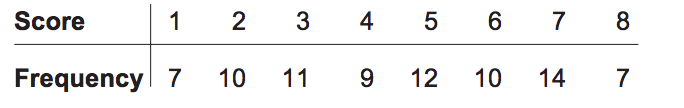
\includegraphics{octo_die.png}
\end{center}

\begin{tight_enumerate}
  \item $G$
  \item Multiple Proportions (Goodness of Fit)
  \item Bar graph
  \item $H_a:$ observed proportions $\ne$ hypothesized proportions (from hypothesized distribution)
  \item $X^2 \sim \chi^2 (df = 8 - 1 = 7)$
\end{tight_enumerate}

\end{document}
